% ****** Start of file aipsamp.tex ******
%
%   This file is part of the AIP files in the AIP distribution for REVTeX 4.
%   Version 4.1 of REVTeX, October 2009
%
%   Copyright (c) 2009 American Institute of Physics.
%
%   See the AIP README file for restrictions and more information.
%
% TeX'ing this file requires that you have AMS-LaTeX 2.0 installed
% as well as the rest of the prerequisites for REVTeX 4.1
% 
% It also requires running BibTeX. The commands are as follows:
%
%  1)  latex  aipsamp
%  2)  bibtex aipsamp
%  3)  latex  aipsamp
%  4)  latex  aipsamp
%
% Use this file as a source of example code for your aip document.
% Use the file aiptemplate.tex as a template for your document.
\documentclass[%
 aip,
% jmp,
% bmf,
% sd,
% rsi,
 amsmath,amssymb,
preprint,%
 %reprint,%
%author-year,%
%author-numerical,%
% Conference Proceedings
]{revtex4-1}
%4 added pacakges
\usepackage{physics}
\usepackage{import}

\usepackage{graphicx}% Include figure files
\usepackage{dcolumn}% Align table columns on decimal point
\usepackage{bm}% bold math
%\usepackage[mathlines]{lineno}% Enable numbering of text and display math
%\linenumbers\relax % Commence numbering lines

\usepackage[utf8]{inputenc}
\usepackage[T1]{fontenc}
\usepackage{mathptmx}
\usepackage{etoolbox}

%% Apr 2021: AIP requests that the corresponding 
%% email to be moved after the affiliations
\makeatletter
\def\@email#1#2{%
 \endgroup
 \patchcmd{\titleblock@produce}
  {\frontmatter@RRAPformat}
  {\frontmatter@RRAPformat{\produce@RRAP{*#1\href{mailto:#2}{#2}}}\frontmatter@RRAPformat}
  {}{}
}%
\makeatother
\begin{document}

\preprint{AIP/123-QED}

\title[Sample title]{Sample Title:\\with Forced Linebreak}
% Force line breaks with \\
\author{C. A. Cartagena-Sanchez}
\email{ccartagena@brynmawr.edu}

 \affiliation{Physics Department, Bryn Mawr College
 }%Lines break automatically or can be forced with \\
\author{D. A. Schaffner}%
 %\email{Second.Author@institution.edu.}
\affiliation{Physics Department, Bryn Mawr College
}

\author{J. M. Carlson}
\affiliation{Physics Department, Bryn Mawr College
}
\date{\today}% It is always \today, today,
             %  but any date may be explicitly specified

\begin{abstract}
\textit{This abstract needs to be updated for the paper.}\\
Turbulent magnetic fluctuations are ubiquitous in both astrophysical and laboratory plasmas that exhibit power-law broadband fluctuations and intermittency. Power-law like broadband fluctuations indicate an energy-cascade where energy is injected at large scales and cascades to smaller and smaller scales where energy is ``dissipated'' via some mechanism. Intermittency in the magnetic fluctuations is associated with current sheets or coherent structures. This talk focuses on understanding the dissipation scale and the intermittent behavior of the magnetic fluctuations. The fluid Taylor scale is investigated as a potential dissipation scale. The Taylor scale is obtained through multi-point correlations of broadband fluctuations. From the spatial and temporal correlations respectively, the measured Taylor scales are $2\pm1cm$ and $3\pm1cm$. Intermittency in magnetic fluctuations is investigated through a statistical analysis of temporal and spatial increments: the probability density function of increments and its moments, i.e. structure functions.
\end{abstract}

\maketitle

\section{For Whom am I writing for?}
I am writing for new graduate students entering the field of plasma turbulence.\\

\begin{figure}
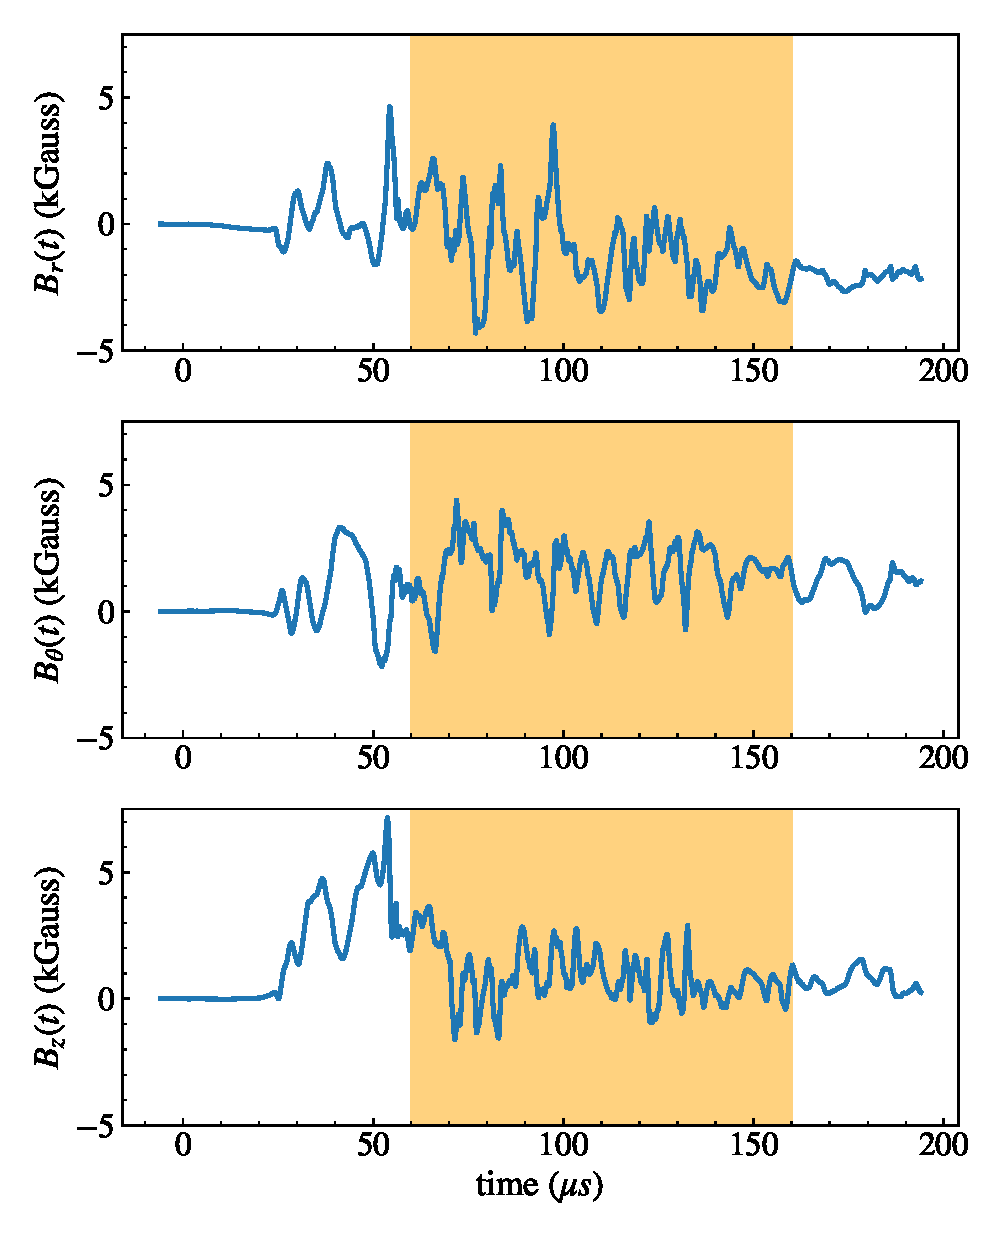
\includegraphics[width=0.65\textwidth]{Figures/fields/bfields_time_num20.pdf}% Here is how to import EPS art
\caption{\label{fig:wave_psd} The magnetic fields measured at $z = 41.6cm$. The highlighted region is the analysis region.}
\end{figure}

What is the Taylor scale in a turbulent laboratory plasma?
The Taylor scale in a turbulent laboratory plasma is $\sim4.6cm$.\\

Does the Taylor scale correspond to dissipation features in the spectra?
The Taylor scale corresponds to a steepening expected in dissipation.
\begin{figure}
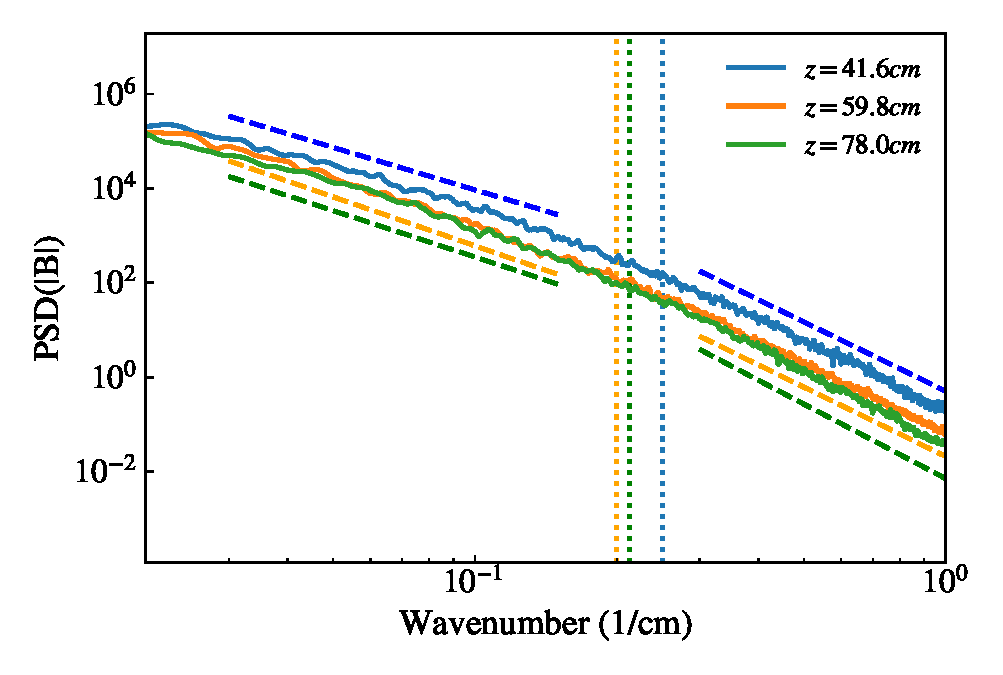
\includegraphics[width=0.65\textwidth]{Figures/psd/pwr_den_k_interp_all_window_lmfit.pdf}% Here is how to import EPS art
\caption{\label{fig:wave_psd} The $|\vb{B}|$ wavenumber power spectral density at three positions: $41.6cm$, $59.8cm$, and $78.0cm$. I used the Taylor scale to partition the wavenumber power spectral density into two regions. The spectral index steepens on average from $-3.2$ to $-5.0$.}
\end{figure}
\\

Is intermittency observed in the magnetic fluctuations?
Intermittency is present in the magnetic fluctuations.\\

\begin{figure}
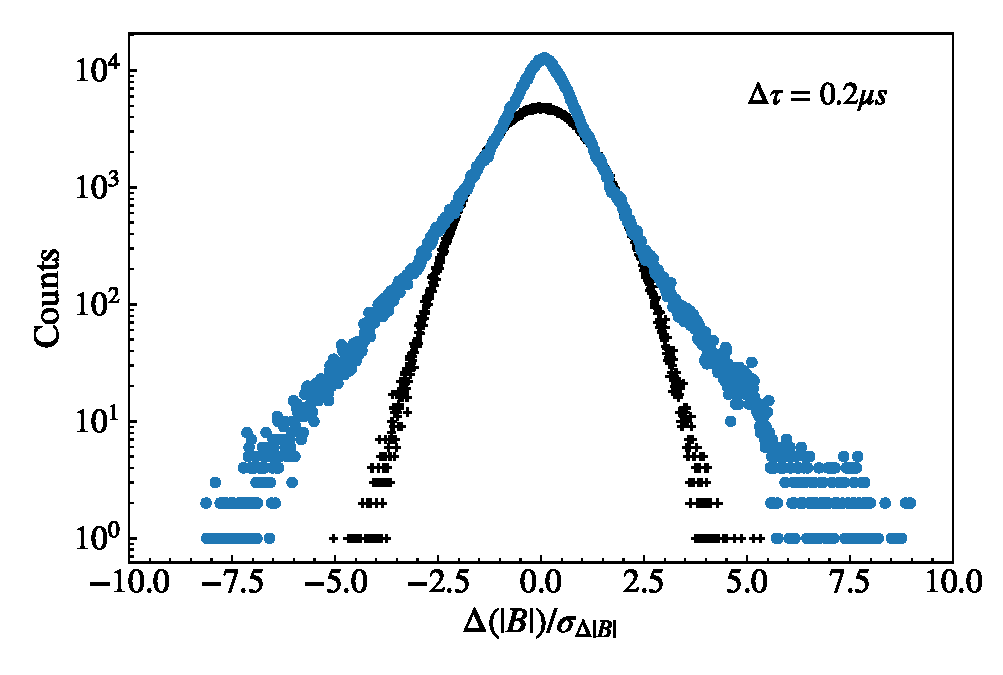
\includegraphics[width=0.65\textwidth]{Figures/Intermittency_figs/new_avg_incr_hist_counts_0.2us_with_rand_p5.pdf}% Here is how to import EPS art
\caption{\label{fig:intermit_0.2} The histogram of $0.2\mu s$ increments. The histogram deviates from a Gaussian histogram, $0.2\mu s$ increments from random data. This features indicates that intermittency is present in the magnetic fluctuations.}
\end{figure}


Is there spacial variation in intermittency?
Intermittency does not appear to vary spatially statistically.\\

\begin{figure}
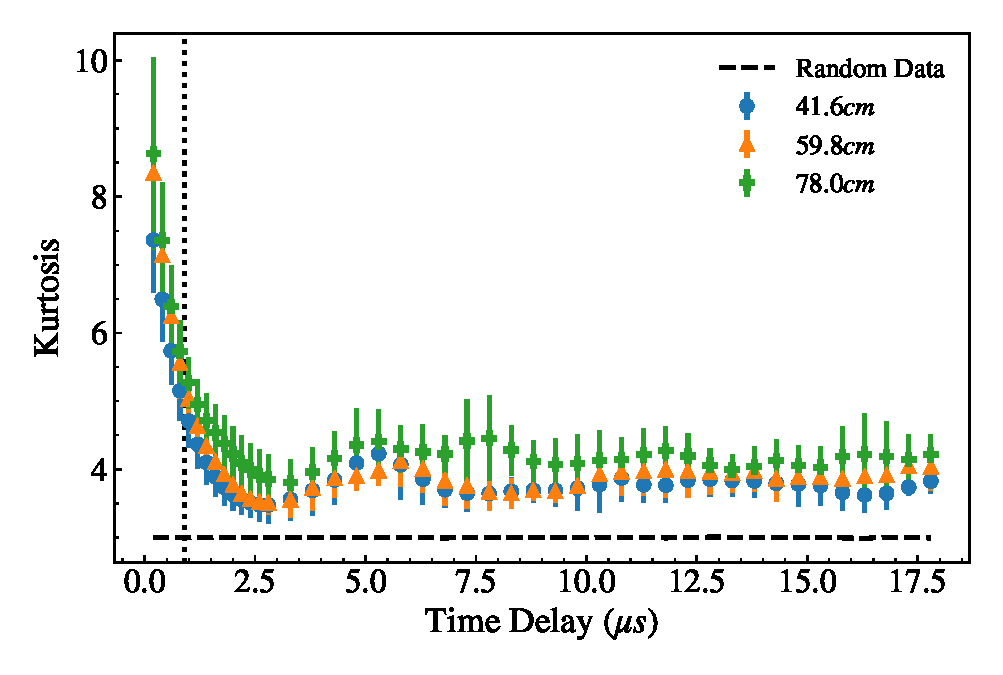
\includegraphics[width=0.65\textwidth]{Figures/Intermittency_figs/ensem_merge_kurt_10shot_range_all_with_rand_tscales.pdf}% Here is how to import EPS art
\caption{\label{fig:kurtosis} The kurtosis measurements of various ensembles of increments, and at the three axial positions: $41.6cm$, $59.8cm$, and $78.0cm$. There is insignificant spatial variation of the kurtosis.}
\end{figure}
\bibliography{aipsamp}% Produces the bibliography via BibTeX.



\end{document}
%
% ****** End of file aipsamp.tex ******